\section{Fallstudie Grundlagen}

\subsection{Minimaler Kernel bauen}

Als erster Schritt soll der Kernel selber kompiliert werden. Versuchen Sie ein möglichst
kleines Image zu erstellen, indem Sie Optionen abschalten. Erstellen Sie zunächst eine 
Konfiguration über \emph{Menuconfig} und messen Sie anschliessend die Dauer des Kompilierens und
die Grösse des Images.

\begin{lstlisting}
$ cd linux-source
$ make menuconfig
\end{lstlisting}

Die Navigation erfolgt über die Pfeiltasten. Mit der Leertasten können Optionen an- bzw. abgewählt werden
und mittels der Tabulatortaste kann der Fokus verändert werden. \\

Kompilieren Sie nun den Kernel und messen sie mit \emph{time} die Dauer. Schreiben Sie alle Zeiten auf (\emph{real}, \emph{user}, \emph{sys}).
Mit dem Unix-Tool \emph{du} (Disk usage) kann die Grösse des Images gemessen werden.

\begin{lstlisting}
$ time make
make[1]: Nothing to be done for 'all'.
  HOSTCC  scripts/basic/fixdep
  HOSTCC  arch/x86/tools/relocs_32.o
  HOSTCC  arch/x86/tools/relocs_64.o
  HOSTCC  arch/x86/tools/relocs_common.o
  HOSTLD  arch/x86/tools/relocs
[...]
real  XXmX.XXXs
user  XXmX.XXXs
sys   XXmX.XXXs

$ du -h arch/x86/boot/bzImage 
X.XM  arch/x86/boot/bzImage

\end{lstlisting}
\hfill

Ergebnisse eintragen:
\begin{tabbing}
 \hspace{1cm}   \= real \hspace{0.2cm} \= \underline{\hspace{0.4cm}}m\underline{\hspace{0.4cm}}.\underline{\hspace{0.6cm}}s \= \hspace{0.2cm} bzImage \underline{\hspace{0.4cm}}.\underline{\hspace{0.2cm}}M \\
                \> user                \> \underline{\hspace{0.4cm}}m\underline{\hspace{0.4cm}}.\underline{\hspace{0.6cm}}s  \\
                \> sys                 \> \underline{\hspace{0.4cm}}m\underline{\hspace{0.4cm}}.\underline{\hspace{0.6cm}}s 
\end{tabbing}

Wie könnte die Imagegrösse weiter verkleinert werden bzw. was hat alles einen Einfluss?

\underline{\hspace{\textwidth}}


\subsection{Kernel-Modul erstellen}

Erstellen Sie nun ein eigenes Kernel-Modul. Legen Sie dafür die Ornderstruktur
wie in Abbildung \ref{fig:basic_dirs} an.
\clearpage

\begin{figure}[h!]
   \begin{center}
      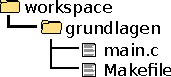
\includegraphics{images/basic_dirs}
   \end{center}
   \caption{Ordnerstruktur}
   \label{fig:basic_dirs}
\end{figure}

Nehmen Sie dazu das Codebeispiel aus der Vorlesung und kopieren Sie
dieses in das \emph{main.c} und füllen Sie das Makefile mit folgendem Inhalt:

\begin{lstlisting}[caption=Makefile]
MODULE_NAME = grundlagen
SRC := main.c

KDIR := /lib/modules/$(shell uname -r)/build

obj-m := $(MODULE_NAME).o
$(MODULE_NAME)-objs = $(SRC:.c=.o)

PWD := $(shell pwd)

all:
   $(MAKE) -C $(KDIR) M=$(PWD) modules

clean:
   $(MAKE) -C $(KDIR) M=$(PWD) clean

\end{lstlisting}

Kompilieren Sie nun das Modul.
\begin{lstlisting}
$ make
\end{lstlisting}

Laden Sie das Modul mit \emph{insmod} (Install module).
\begin{lstlisting}
$ sudo insmod grundlagen.ko
\end{lstlisting}

Entladen Sie das Modul mit \emph{rmmod} (Remove module).
\begin{lstlisting}
$ sudo rmmod grundlagen.ko
\end{lstlisting}

Die Ausgaben von \emph{printk()} werden ins Kernellog geschrieben. Sie können das Kernellog mit \emph{dmesg} (Dump messages) anzeigen lassen.
\begin{lstlisting}
$ dmesg | tail -n 10
\end{lstlisting} \hfill

Was steht im Kernellog? \\

[00000.000000] \underline{\hspace{0.5\textwidth}} \newline
[00000.000000] \underline{\hspace{0.5\textwidth}} \newline
[00000.000000] \underline{\hspace{0.5\textwidth}} \newline
[00000.000000] \underline{\hspace{0.5\textwidth}} \newline
[00000.000000] \underline{\hspace{0.5\textwidth}} \newline
[00000.000000] \underline{\hspace{0.5\textwidth}} \newline
[00000.000000] \underline{\hspace{0.5\textwidth}} \newline
[00000.000000] \underline{\hspace{0.5\textwidth}} \newline
[00000.000000] \underline{\hspace{0.5\textwidth}} \newline
[00000.000000] \underline{\hspace{0.5\textwidth}} \newline

\subsection{Log-Level}

Ersetzen Sie das Log-Level in \emph{printk()} durch diese in der Tabelle \ref{tab:loglevel}.

\begin{table}[h!]
   \begin{center}
   \begin{tabular}{| l | l |} \hline
   KERN\_DEBUG   & Debuggen (Alle Nachrichten) \\ \hline
   KERN\_INFO    & Informative Nachricht \\ \hline
   KERN\_NOTICE  & Wichtige Information \\ \hline
   KERN\_WARNING & Warnung \\ \hline
   KERN\_ERR     & Fehler \\ \hline
   KERN\_CRIT    & Kritischer Fehler \\ \hline
   KERN\_ALERT   & Fehlerbehebung muss sofort erfolgen \\ \hline
   KERN\_EMERG   & System ist nicht mehr benutzbar \\ \hline
   \end{tabular}
   \caption{Log-Levels}
   \label{tab:loglevel}
   \end{center}
\end{table}


Wie verhalten sich die Log-Levels? Vergleichen Sie dabei die Ausgabe im Kernellog.

\underline{\hspace{\textwidth}}
